\subsection{Use Case}
\label{sec:usecase}

The use cases in figure \ref{tab:actoreventtable} are described below.  

\paragraph{See all problems} The use case see all problem is used by both \aclient{} and \astaff{}. It works as a searchable list. 

\paragraph{\bloadwork[c]} \bloadwork[c] is the operation of the \wmon{}. It checks and compares all staff members workload and redistribute problems in order to equally balance the workload in each department. 

\paragraph{\gstat[c]} The use case \gstat[] is trivial and is a list of different views each showing a kind of statistics. The use case can be accessed by \sadmin{}, \aclient{}, and \astaff{}, but they cannot access all the same statistics.

\paragraph{\ucsproblem[c]} The use case \ucsproblem[] is only used be the actor \aclient. Except for cases when \astaff{} or \sadmin{}  acts as \aclient{}. A use case diagram is shown in figure \ref{fig:submit_problem_use_case}. 
\begin{itemize}
\item \sadb{Use Case:} \ucsproblem[c] is initialized when a \aclient{} has a problem and wishes to submit that problem to the system in order to get help from the \astaff{}. 
He first has to select a category and from that choose one or more tags, he can change category and select even more tags. 
When the \aclient{} is done selecting tags the system compares the selected tags with other problems. 
If similar problems is found the \aclient{} is presented with these.
If one of these matches his particular problem, he can subscribe to the problem(if \open), reopen problem(if \closed{})\fixme{Udem\ae{}rket her, vi skal bare huske at den i stedet laver et nyt problem}, or use the information in the old problem to solve his problem independently. 
If no similar problem was found the \aclient{} creates a problem with a description and the previously selected tags. 
Hereafter the problem gets assigned to a \astaff{}. 

\item \sadb{Objects:} Problem, solution, tag, category, \client, \staff. (Department)\fixme{Hvad betyder det at den er i parentes}

\item \sadb{Functions:} Search existing problems, compare problems, create problem, attach user to problem.
\end{itemize}

%%%%%%%%% BEGIN COMMENT
\begin{comment}
\begin{sadlist}[h]{\ucsproblem[c]}{Description of the use case submit problem.}{fig:ucsproblem}
\sadb{Use Case:} \ucsproblem[c] is initialized when a \aclient{} has a problem and wishes to submit that problem to the system in order to get help from the \astaff{}. 
He first has to select a category and from that choose one or more tags, he can change category and select even more tags. 
When the \aclient{} is done selecting tags the system compares the selected tags with other problems. 
If similar problems is found the \aclient{} is presented for the problems.
if one of these matches his particular problem, he can subscribe to the problem(if \open), reopen problem(if \closed{}), or use the information in the old problem to solve his problem independently. 
If no similar problem were found the \aclient{} creates a problem with a description and the previously selected tags. 
Hereafter the problem gets assigned to a \astaff{}. 

\sadb{Objects:} Problem, solution, tag, category, \client, \staff. (Department)

\sadb{Functions:} Search existing problems, compare problems, create problem, attach user to problem.
\end{sadlist}
\end{comment}
%%%%%%%%%% END COMMENT



\begin{figure}[htbp]
\begin{center}
 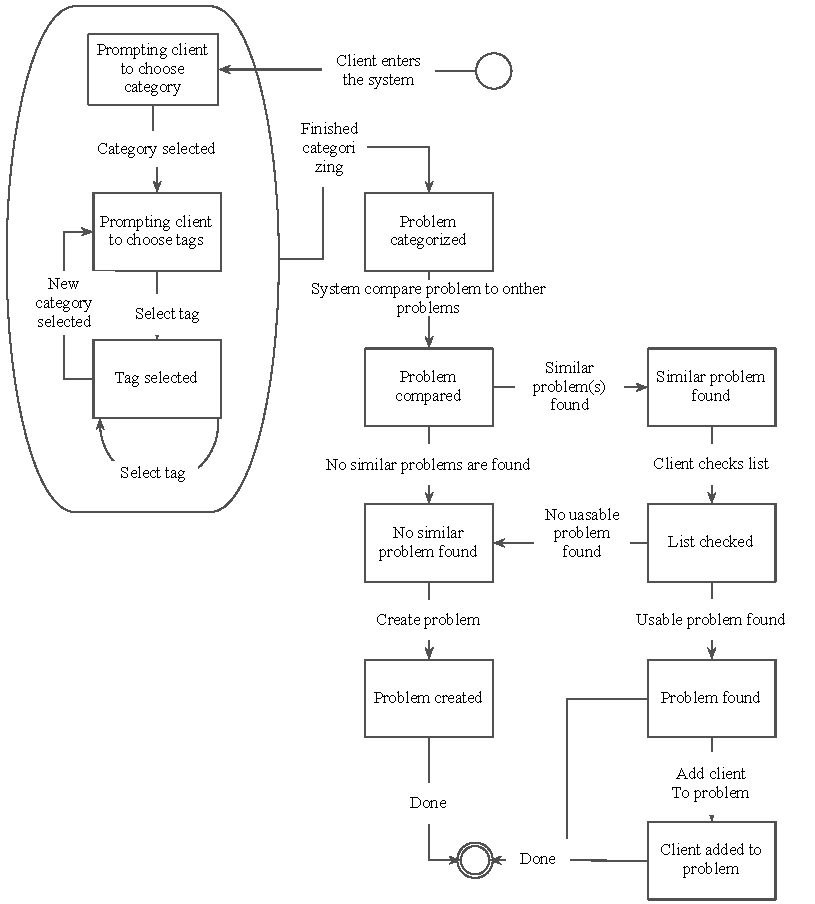
\includegraphics[scale=0.8]{input/application_domain_analysis/submit_problem_use_case}
\morscaption{A state chart diagram of the use case \ucsproblem{}.}
\label{fig:submit_problem_use_case}
\end{center}
\end{figure}



\paragraph{\ucsolproblem[c]} The use case \ucsolproblem{} is the \astaff{}s primary working usage of the system. This is where he goes to get his \todolist{} and to solve problems. A diagram is shown in figure \ref{fig:solve_problem_use_case}.

\begin{itemize}
\item \sadb{Use Case:} The use case is initialized when the \astaff[] wants to check his \todolist[]. He is then presented with a list of unsolved problems assigned to him. He can then click on one of the problems to solve the problem, see status of it, add comments to it, search the database for similar problem, reassign it, or delete it. 

\item \sadb{Objects:} Problem, solution, tag, category, comment, \client[], \staff[] and department. 

\item \sadb{Functions:} Add comment, reassign, change status, delete problem, search database, create solution, attach solution and get staff \todolist{}.
\end{itemize}


%%%%%%%%%%%%% BEGIN COMMENT
\begin{comment}
\begin{sadlist}[htb]{\ucsolproblem[c]}{Description of the use case \ucsolproblem{}.}{fig:ucsolproblem}
\sadb{Use Case:} The use case is initialized when the \astaff[] wants to check his \todolist[]. He is then presented with a list of unsolved problems assigned to him. He can then click on one of the problems to solve the problem, see status of it, add comments to it, search the database for similar problem, reassign it or delete it. 

\sadb{Objects:} Problem, solution, tag, category, comment, \client[], \staff[] and department. 

\sadb{Functions:} Add comment, reassign, change status, delete problem, search database, create solution, attach solution and get staff \todolist{}.
\end{sadlist}
\end{comment}
%%%%%%%%%%%%%%% END COMMENT

\begin{figure}[htbp]
\begin{center}
 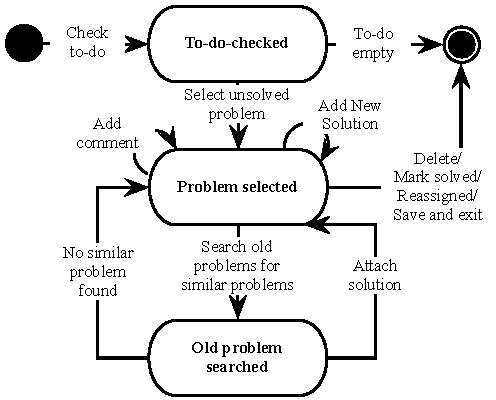
\includegraphics[scale=0.8]{input/application_domain_analysis/solve_problem_use_case}
\morscaption{A state chart diagram of the use case \ucsolproblem{}.}
\label{fig:solve_problem_use_case}
\end{center}
\end{figure}


\paragraph{\tucadmin[c]} The use case \tucadmin[] is used by the \sadmin[] to administrate persons, tags, categories and departments. A statechart diagram is depicted on figure \ref{fig:use_case_diagram}.

\begin{itemize}
\item\sadb{Use Case:} The use case starts as the \sadmin{} enters the site. He can add/remove persons and departments. The \sadmin{} can select departments and from the selected department he can add or remove \staff[]s and categories. From both a selected department and the main window he can select a person to edit. 
If he selects a department he can select a category to change and from that category select, add, and remove tags. 
From a selected tag the \sadmin{} can set/change the priority of the specific tag. From any point he can go back or leave the administration. 

\item\sadb{Objects:} \staff[c], \client[c], category, tag, department.

\item\sadb{Functions:} Delete person, Add person, create department, set permissions, delete department, set priority, add category, delete category, set tag visibility, set category visibility, create tag, delete tag.
\end{itemize}



%%%%%%%%%%%% BEGIN COMMENT
\begin{comment}
\begin{sadlist}[h]{\tucadmin[c]}{Description of the use case \tucadmin{}.}{fig:tucadmin}
\sadb{Use Case:} The use case starts as the \sadmin{} enters the system. He can add/remove users and depertments. The \sadmin{} can select departments and from the select department add or remove staffs and categories. He can from the department select a category to change and from that category select, add, and remove tags. From a selected tag the \sadmin{} can set/change the priority of the specific tag. From any point he can go back or leave the administration. 

\sadb{Objects:} \staff[c], \client[c], category, tag, department.

\sadb{Functions:} Remove user, remove client, add client, add staff, create department, delete department, set priority, add category, delete category, set tag visibility, set category visibility, create tag, delete tag.

\end{sadlist}
\end{comment}
%%%%%%%%%%%%%% END COMMENT

\begin{figure}[htbp]
\begin{center}
 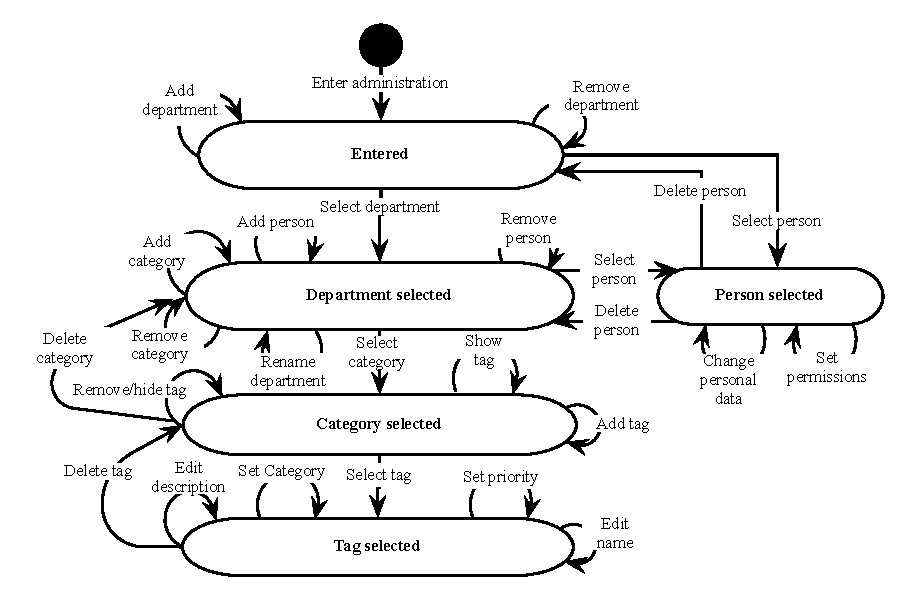
\includegraphics[scale=0.8]{input/application_domain_analysis/admin_use_case}
\morscaption{A statechart diagram for the use case \tucadmin{}.}
\label{fig:use_case_diagram}
\end{center}
\end{figure}